%% Beispiel-Präsentation mit LaTeX Beamer im KIT-Design
%% entsprechend den Gestaltungsrichtlinien vom 1. August 2020
%%
%% Siehe https://sdqweb.ipd.kit.edu/wiki/Dokumentvorlagen

%% Beispiel-Präsentation
\documentclass[en]{sdqbeamer}
\usepackage{algorithm}
\usepackage{algpseudocode}
 
\newcommand\blfootnote[1]{%
  \begingroup
  \renewcommand\thefootnote{}\footnote{#1}%
  \addtocounter{footnote}{-1}%
  \endgroup
}

%% Titelbild
\titleimage{unima_schloss}

%% Gruppenlogo
\grouplogo{} 

%% Gruppenname und Breite (Standard: 50 mm)
\groupname{Mannheim Master Datascience}
%\groupnamewidth{50mm}

% Beginn der Präsentation

\title[HybridBERT4Rec]{HybridBERT4Rec: A Hybrid Recommender System Based on BERT}
\subtitle{Sequential Content-Based and Collaborative Filtering}
\author[Leon Knorr]{Leon Knorr}

\date[\today]{\today}

% Literatur 
 
\usepackage[citestyle=numeric,bibstyle=numeric,hyperref,backend=biber]{biblatex}
\addbibresource{sources.bib}
\bibhang1em

\begin{document}
 
%Titelseite
\KITtitleframe

%Inhaltsverzeichnis
\begin{frame}{Table of Contents}
\tableofcontents
\end{frame}

\section{Recap}

\begin{frame}
	\centering\textbf{\LARGE{Recap: Sequential Modelling \& HybridBERT4Rec}}
\end{frame}

\subsection{Sequential Modelling}
\begin{frame}{Traditional CBF VS Sequential CBF}
	\begin{columns}
	\column{0.5\textwidth}
		\begin{figure}
			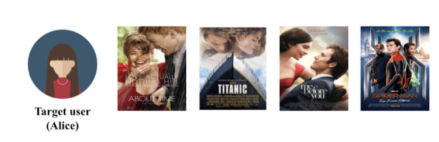
\includegraphics[width=\textwidth]{images/Alice_history.pdf}
			\caption{Example history for Alice in traditional CBF \cite{channarongHybridBERT4RecHybridContentBased2022}}
		\end{figure}
		\begin{itemize}
			\item models \textbf{general} user preference \pause
			\item \textbf{BUT:} User preferences \underline{\textbf{change over time!}} \cite{wangSequentialRecommenderSystems2019}
		\end{itemize}

	\column{.5\textwidth}
		\begin{figure}\pause
			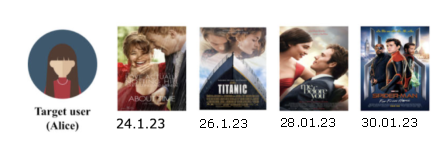
\includegraphics[width=\textwidth]{images/Alice_seq.pdf}
			\caption{Example history for Alice in sequential CBF \cite{channarongHybridBERT4RecHybridContentBased2022}}
		\end{figure}
		\begin{itemize}
			\item Considers the \textbf{order} of historical interactions
			\item Allows the modelling of \enquote{temporary spikes} of interests, as well as the general preferences \cite{wangSequentialRecommenderSystems2019}
		\end{itemize}
	\end{columns}
\end{frame}

\subsection{HybridBERT4Rec}
\begin{frame}{HybridBERT4Rec Architecture}
	\begin{figure}
		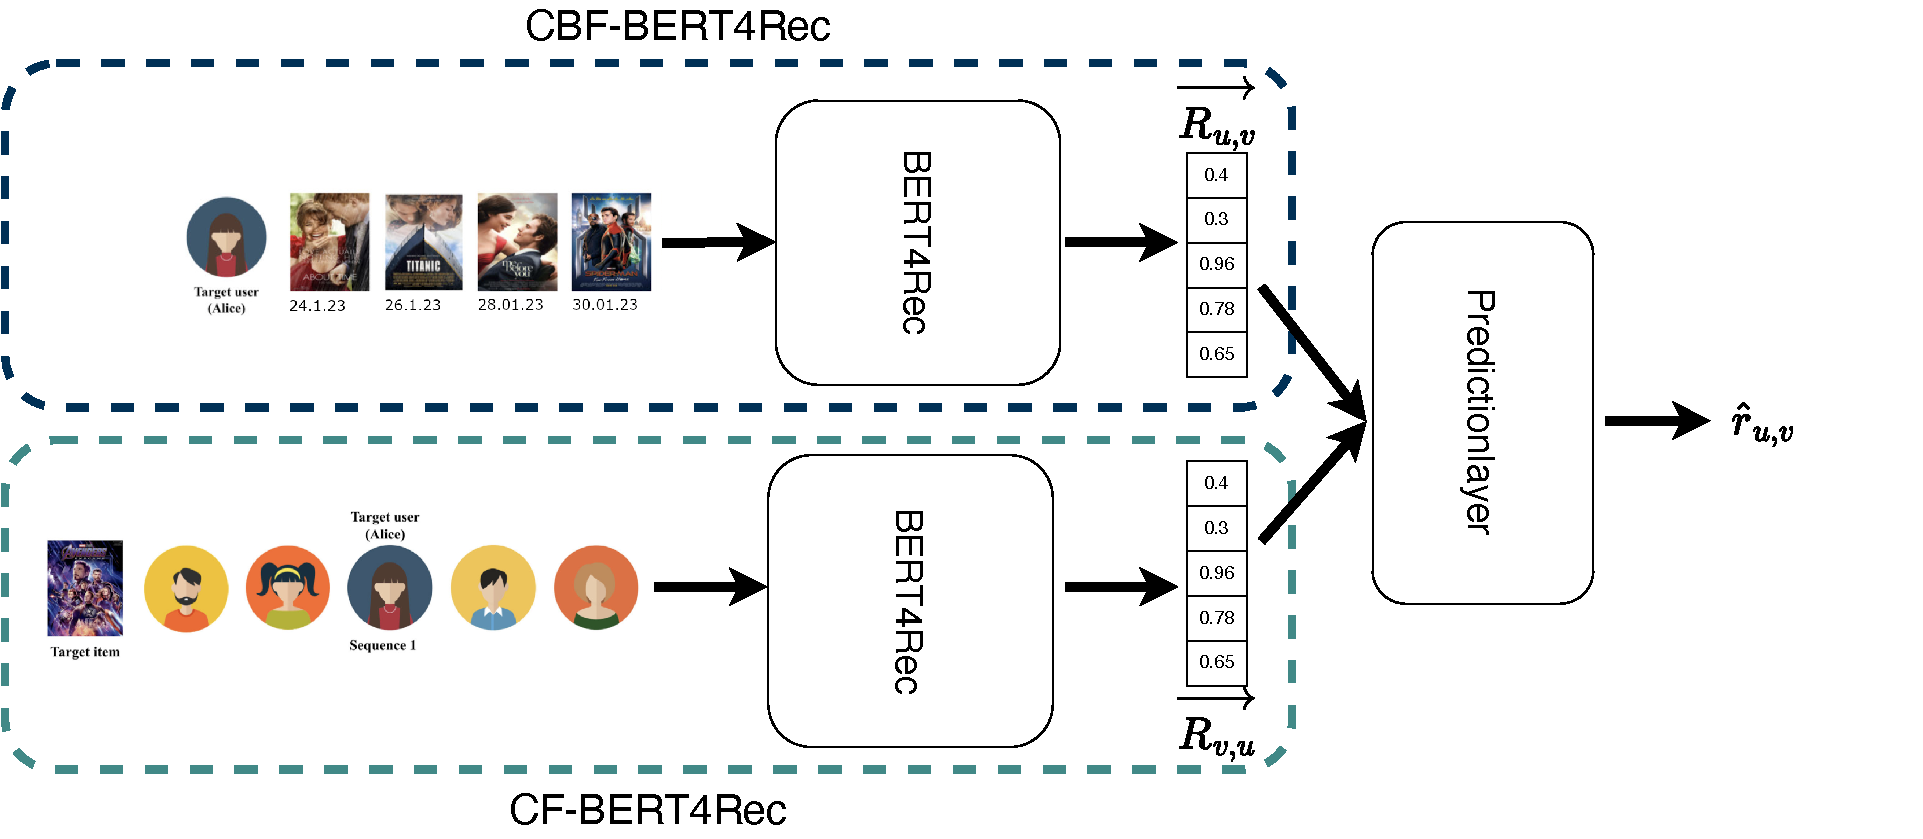
\includegraphics[height=0.6\textheight]{images/hybridBERT4Rec_high_level.pdf}
		\caption{High level overview of HybridBERT4Recs Architecture. \cite{channarongHybridBERT4RecHybridContentBased2022}}
	\end{figure}
\end{frame}

\section{The Setting}

\begin{frame}
	\centering\textbf{\LARGE{The Setting}}
\end{frame}

\begin{frame}{The Setting}
	\begin{figure}
		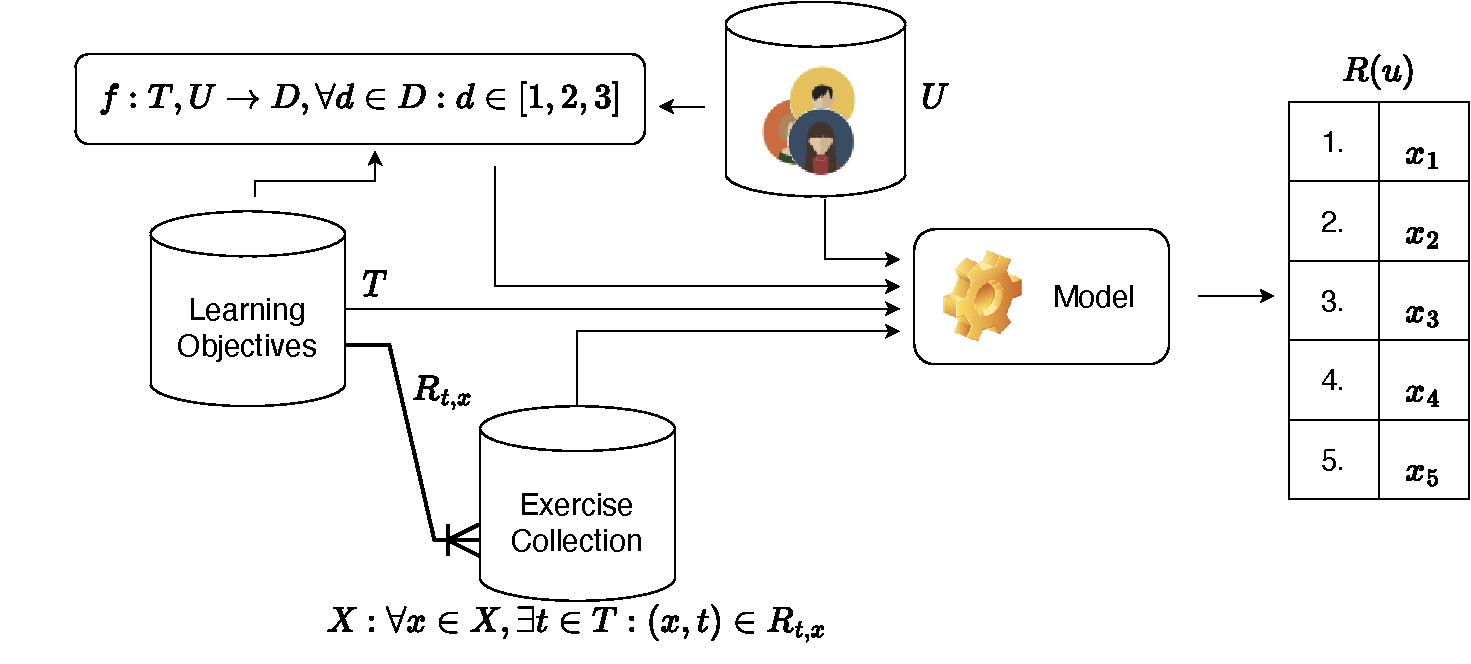
\includegraphics[height=0.6\textheight]{images/setting.pdf}
		\caption{The Setting, consisting of a user collection $U$ and their histories $h(u)$, a collection of learning objectives $T$ and a collection of exercises $X$, which can be used to predict a ranking $R(u)$ for a given user $u$.}
	\end{figure}
\end{frame}

\section{Model Adaption}
\begin{frame}
	\centering\textbf{\LARGE{Model Adaption}}
\end{frame}

\begin{frame}{CBF-HybridBERT4Rec}
	\begin{columns}
		\column{0.5\textwidth}
			\begin{itemize}
				\item $H(u) := (\{(x_i, t_j, s_k)| (x_i, t_j) \in R_{t,x}\}, \leq)$, with $s_{k-1} \leq s_k$
				\item $I(u) := (\{x_i|(x_i, t_j, s_k) \in H(u)\}, \leq)$
				\item $\overrightarrow{R_{u,t}}$: the interaction probability distribution of all items with the user $u$ over the target item
			\end{itemize}
		\column{0.5\textwidth}
		\begin{figure}
			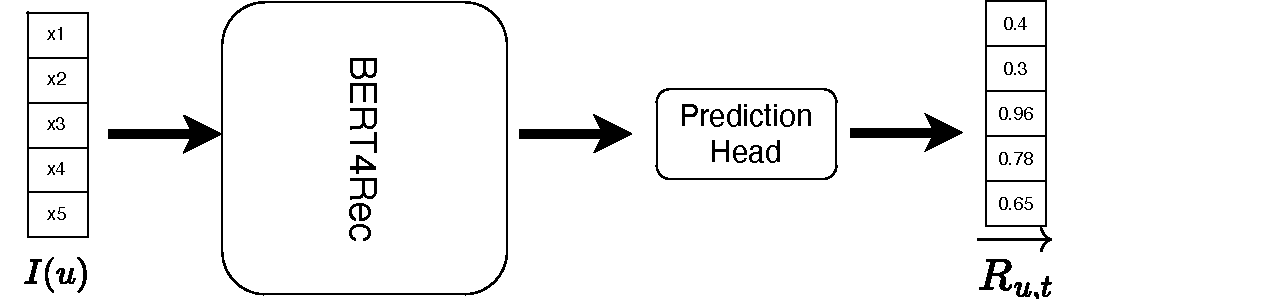
\includegraphics[width=\textwidth]{images/cbf.pdf}
			\caption{CBF-HybridBERT4Rec architecture and input in the described setting}
		\end{figure}
	\end{columns}
\end{frame}

\begin{frame}{CF-HybridBERT4Rec}
	\begin{columns}
		\column{0.5\textwidth}
			\begin{itemize}
				\item $u \in N \iff d_{u, t} = d_{u_m, t} \, \wedge$ $(x, t) \in \{(x,t)|(x,t,s_k) \in H(u)\}$, with $U_m \in U, U \in U, t \in T$, $N$ being the set of neighbors for target (masked) user $u_{m}$ and learning objective $t$
				\item $\overrightarrow{R_{t,u}}$: a user-similarity probability distribution of all users over the target (masked) user
			\end{itemize}
		\column{0.5\textwidth}
		\begin{figure}
			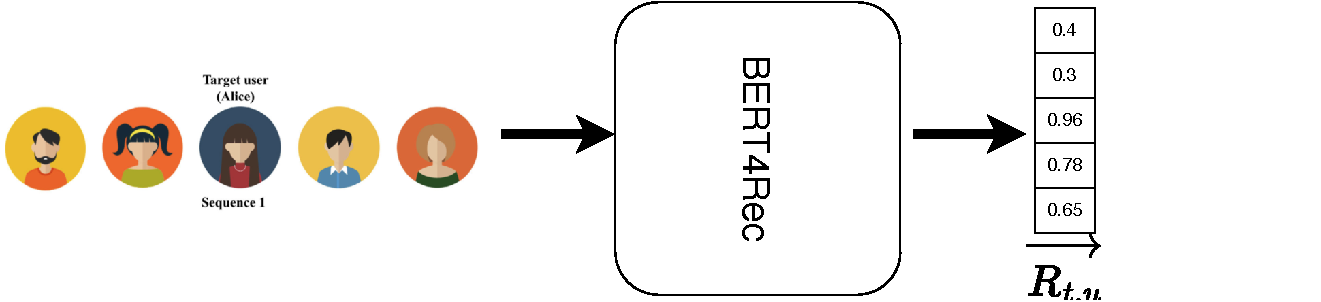
\includegraphics[width=\textwidth]{images/CF_use_case.pdf}
			\caption{CF-HybridBERT4Rec architecture and input in the described setting}
		\end{figure}
	\end{columns}
\end{frame}

\begin{frame}{Bringing It All Together}
	\begin{columns}
		\column{0.5\textwidth}
		\begin{algorithm}[H]
			\caption{HybridBERT4Rec in an E-Learning Setting}
			\begin{algorithmic}[1]
				\ForAll{$u_m \in U$}
					\State $r_{x,u_m} = \texttt{cbf\_hybridbert4rec}(H(u_m))$
					\ForAll{$(x,t) \in R_{t,x}$}
						\State $r_{u, x} = \texttt{cf\_bert4rec}(u_m,t,x)$
						\State $\hat{r}_{u,x} = \texttt{prediction\_layer}(r_{x,u}, r_{u,x})$
					\EndFor
				\EndFor
			\end{algorithmic}
		\end{algorithm}
		\column{0.5\textwidth}
		\begin{itemize}
			\item Yields a rating $\hat{r}_{u,x}$ for each exercise and for each user
			\item Construct an overall rating of exercises by sorting the ratings
			\item Construct a topic specific rating by filtering for a topic and sorting the ratings
		\end{itemize}
	\end{columns}
\end{frame}

\section{Evaluation}
\begin{frame}
	\centering\textbf{\LARGE{Evaluation}}
\end{frame}
\begin{frame}{The Problem}
	\begin{itemize}
		\item No given Test data with relevance annotations!
		\item Annotating the whole collection requires $U \times T \times X$ relevance annotations
		\item \textbf{INFEASIBLE} for large $U, X$ and $T$
	\end{itemize}
\end{frame}
\begin{frame}{Pooling}
	\begin{itemize}
		\item For most queries only $N << X$ documents are relevant
		\item[$\Rightarrow$] We only annotate the top $N$ results of every query
		\item[$\Rightarrow$] $U \times T \times N$ relevance annotations needed
		\item Compute P@K, R@K, NDCG etc.
		\item \textbf{Shortcoming}: Scores are only \textbf{approximations!}
	\end{itemize}
\end{frame}

\appendix
\beginbackup
\begin{frame}{References}
	\printbibliography
\end{frame}

\backupend

\end{document}